\chapter{Exploration: Regret and Multi-Armed bandits}

The exploration-exploitation problem is about making choices when you're not sure what's best.
Imagine you have to pick between something you already know works well (exploitation) or trying something new that could be better or worse (exploration).
If you always stick to what you know, you might miss out on better options.
But if you keep trying new things, you might waste time on things that don’t work.
The trick is to find a balance: sometimes try new things, but also use what you've already learned works well.

\section{Multi-armed Bandit}

The exploration-exploitation problem is difficult to solve in complex scenarios, so we simplify it to make the analysis more manageable. The multi-armed bandit setting is chosen because it offers a simple and clear framework for this problem.

The multi-armed bandit problem is a decision-making problem in which an agent is faced with multiple actions (arms), each providing a reward based on an unknown probability distribution. The goal of the agent is to maximize the total reward over a series of trials by balancing two strategies:

\begin{itemize}
    \item Exploitation: Selecting the arm that has given the highest rewards so far.
    \item Exploration: Trying different arms to gather more information about their potential rewards.
\end{itemize}

There are $K$ different arms $a_1, \dots, a_K$. Each arm $a_i$ has an unknown reward distribution $\nu_i$, with an expected reward $\mathbb{E}_{r \sim \nu_i}[r] = \mu_i$. At each time step $t$, the agent selects an arm $a_t$ and receives a reward $r_t$, where $r_t$ is sampled from the distribution $\nu_{a_t}$ of the selected arm. The rewards are independent and identically distributed (i.i.d.) for each arm.

The objective is to maximize the cumulative reward over $T$ trials, typically expressed as minimizing the regret, which is the difference between the reward of an optimal policy and the reward accumulated by the agent.

We can think of a reward as a form of feedback because it provides information about the outcome of a choice (i.e., pulling an arm). When you pull an arm, the reward indicates whether that choice was beneficial or not. A high reward suggests the arm might be a good choice, while a low reward suggests the arm might not be as favorable. This feedback informs future decisions by helping the agent understand the consequences of its actions.

Since rewards are random and can vary each time you pull an arm, we consider the expectation over the rewards for a given arm. Some pulls might yield high rewards, while others may give low rewards, even though the arm has an underlying expected performance. To reliably evaluate the quality of an arm, we use the expected reward, which represents the average outcome you would obtain if you pulled the arm many times. This expected value gives a more accurate measure of the arm's performance over time, rather than relying on individual outcomes that may be influenced by randomness.

\subsection{Regret}

Regret in the context of the multi-armed bandit problem is a measure of the opportunity loss experienced by not always choosing the best possible action (arm).
It represents the difference between the reward you could have earned by always selecting the optimal arm and the reward you actually received by making imperfect choices.

Formally, regret after $T$ trials is defined as

$$
    R(T) = T \cdot \mu^* - \sum_{t=1}^{T} \mu_{I_t}
$$

\begin{tipbox}[Tip/Explanation]

    The term $T \cdot \mu^*$ represents the total reward you would obtain if you always chose the best arm (with the highest expected reward $\mu^*$) throughout all $T$ trials. Since the best arm remains the same across the experiment, this reflects the hypothetical scenario where you know the best option from the start and consistently stick to it.

    The term $\sum_{t=1}^{T} \mu_{I_t}$ represents the sum of the expected rewards of the arms you actually pulled during the experiment. At each time step $t$, you pull an arm $I_t$, and this sum reflects the expected rewards based on your actual choices.

    The regret measures how much worse your total reward is compared to the scenario where you always picked the optimal arm. The lower the regret, the closer your decisions are to the optimal strategy, indicating better performance over time.
\end{tipbox}

\begin{warningbox}[Warning]
    In the multi-armed bandit problem, both $\mu^*$ (the expected reward of the best arm) and $\mu_{I_t}$ (the expected reward of the chosen arm at time $t$) represent the true underlying reward distributions. However, in practice, we do not have direct access to these true distributions. Instead, we must estimate them based on the observed rewards from pulling the arms.

    This estimation introduces uncertainty, as the observed rewards are samples from the underlying distributions. The agent must balance two competing objectives:

    - **Exploration**: Pulling less-known arms to gather information about their reward distributions.
    - **Exploitation**: Pulling arms that appear to have high expected rewards based on the information gathered so far.

    The challenge lies in finding the right balance between these strategies to maximize the cumulative reward over time.

\end{warningbox}

\section{Algorithms for minimizing regret in Multi-Armed bandits}

Now that we have defined the multi-armed bandit (MAB) problem, we can focus on the primary objective: minimizing regret.
In the MAB setting, an agent interacts with multiple arms (choices), each providing rewards drawn from unknown distributions.

At every time step, the agent must decide which arm to pull, aiming to maximize its total reward over time. However, the agent doesn’t know which arm is optimal, so it must balance:

- **Exploration**: Trying different arms to gather information about their reward distributions.
- **Exploitation**: Choosing the best arm based on the information gathered so far.

Minimizing regret means making decisions that come as close as possible to the reward the agent would have earned had it always chosen the best arm from the start. The goal is to reduce the difference between the actual total reward and the hypothetical reward from consistently pulling the optimal arm.

\subsection{Greedy Algorithm}

The idea behind the greedy algorithm is straightforward: it focuses entirely on exploitation. The algorithm works by always selecting the arm that has given the highest reward based on past experiences, without attempting to gather more information (i.e., without exploring).

\begin{enumerate}
    \item Initial Phase: In the very beginning, the agent may try each arm once to get an initial sense of their rewards.
    \item Exploit the Best: After this, the agent commits to always pulling the arm that gave the highest observed reward during the initial phase, assuming that it is the best arm.
\end{enumerate}

This approach is called "greedy" because it chooses the arm that seems best based on the current information, without considering the possibility that there might be better arms that haven’t been sufficiently explored.

\begin{warningbox}[Warning]
    In the case of the greedy algorithm, during the initial phase when the agent tries each arm only once, the mean reward for each arm is based on just a single observed example. This means the decision to exploit (i.e., stick to the arm with the highest observed reward) is made using very limited information.

    Since the mean is taken over only one example, the algorithm might get a skewed sense of which arm is best. For instance, an arm that is actually suboptimal might give a high reward by chance, leading the greedy algorithm to incorrectly exploit that arm for the rest of the trials. As a result, this lack of exploration can cause poor long-term performance, since the agent may prematurely commit to an arm based on misleading early results.
\end{warningbox}

To optimize the decision-making process and avoid suboptimal outcomes from using just one sample, we can improve the greedy algorithm by:

\begin{enumerate}
    \item Try each arm multiple times: By pulling each arm multiple times, we gather more samples of the rewards for each arm. This allows us to better estimate the true expected reward of each arm, reducing the chance that one lucky sample from a suboptimal arm misleads us.

    \item Compute the empirical mean of each arm: The empirical mean is the average reward of the arm based on the samples we've gathered. The more times we pull an arm, the more accurate this estimate becomes, converging toward the true mean reward of that arm as the number of samples increases.

    \item Commit to the arm with the highest empirical mean: After gathering sufficient samples and calculating the empirical means, we can commit to the arm that appears to offer the highest average reward. This balances exploration (trying arms multiple times) with exploitation (choosing the arm that seems best).

\end{enumerate}

\begin{algorithm}
    \caption{Greedy algorithm with empirical mean}
    \begin{algorithmic}[1]
        \State \textbf{Input:} $N$: Number of times to try each arm, $T$: Total number of trials, with $T \gg K$
        \State \textbf{Output:} Sequence containing the arm $I_t$ chosen at each time step $t$

        \For{$k = 1 \dots K$}
        \State Pull the $k$-th arm $N$ times
        \For{$i = 1 \dots N$}
        \State Observe the reward $r_i$
        \EndFor
        \State Compute the empirical mean: $\hat{\mu_k} = \frac{1}{N} \sum_{i=1}^{N} r_i$
        \EndFor

        \State Choose the best empirical arm $I$ as $I = \underset{i \in K}{\arg\max} \, \hat{\mu_i}$

        \For{$t = NK \dots T$}
        \State Pull the best empirical arm $I$
        \EndFor

    \end{algorithmic}
\end{algorithm}

\begin{warningbox}
    The algorithm does not explicitly solve a minimization problem; instead, it reduces regret by ensuring that the best arm is identified and exploited for the remaining trials.
\end{warningbox}

Once the exploration phase is done and you've calculated the empirical means $\hat{\mu}_i$ for all arms, the arm with the highest empirical mean stays fixed and is pulled repeatedly for the rest of the trials. The arm selection is constant during the commitment phase, so the computation of $I_t$ only happens once, not in every iteration of a loop.

\subsubsection{Greedy algorithm regret}


The **Hoeffding Inequality** is a statistical tool that provides a bound on how far the empirical mean $\hat{\mu}$ (the average of observed data) is from the true mean $\mu$ of a probability distribution, given a certain number of i.i.d. samples. In the multi-armed bandit (MAB) context, rewards are assumed to be i.i.d. for each arm.

The empirical mean $\hat{\mu_i}$ of the rewards for an arm is an estimate of the true mean $\mu_i$ of its reward distribution. However, due to the randomness in the rewards, $\hat{\mu_i}$ might not exactly match $\mu_i$. The **Hoeffding Inequality** gives us a confidence interval around the empirical mean, providing a bound on the probability that the difference between the empirical mean $\hat{\mu_i}$ and the true mean $\mu_i$ is within a certain range, depending on the number of samples $N$ and a chosen confidence level $1 - \delta$.

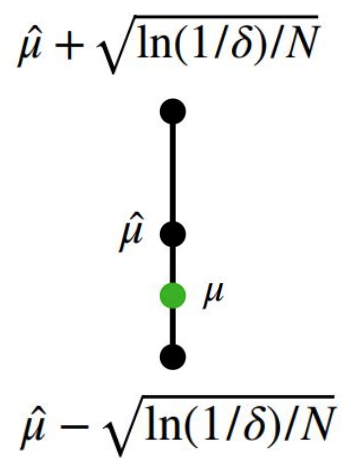
\includegraphics[width=11cm]{Exploration - Regret and Multi-Armed bandits/hoeffding_bounds.png}

During the exploration phase, you are trying out each arm to gather information about their rewards. Since you don't know which arm is the best yet, you will inevitably pull suboptimal arms. Out of the $K$ arms, only one is the best (with the highest reward), and the remaining $(K-1)$ arms are suboptimal.

Let’s assume rewards are either 0 or 1. The worst-case exploration regret is:

$$
    R_{explore}(NK) = NK\mu^* - \sum_{i=0}^NK \hat{\mu_i}
$$

In the worst case, we make the following assumptions:
\begin{itemize}
    \item The optimal arm has a mean reward of 1.
    \item The suboptimal arms have a mean reward of 0.
\end{itemize}

This simplifies the regret to:

$$
    R_{explore}(NK) = NK\mu^* - K \hat{\mu_*}
$$

Where $\hat{\mu_*}$ is our estimate of the optimal arm's mean. We can further simplify this to:

$$
    R_{explore}(NK) = N(K-1) \leq NK
$$

The best empirical arm is chosen as $I = \underset{i \in K}{\arg\max} \, \hat{\mu_i}$. In the worst case, the regret from exploitation can be written as:

$$
    R_{explore}(T-NK) = (T-NK)(\mu_3 - \mu_2)
$$

More generally, we can define:

- The empirical best arm mean:
$$
    \mu_{\hat{I}} = \underset{i \in K}{\arg\max} \, \hat{\mu_i}
$$
- The true best arm mean:
$$
    \mu_{I^*} = \underset{i \in K}{\arg\max} \, \mu_i
$$

Thus, the exploitation regret becomes:

$$
    R_{explore}(T-NK) = (T-NK)(\mu_{I^*} - \mu_{\hat{I}})
$$

To bound $\mu_{I^*} - \mu_{\hat{I}}$, we can use the Hoeffding Inequality:

- The upper bound of $\mu_{I^*}$ is given by the upper confidence bound (UCB):
$$
    \hat{\mu_{I^*}} + \sqrt{\frac{\ln(\frac{K}{\delta})}{N}}
$$

- The lower bound for $\mu_{\hat{I}}$ (to maximize the regret difference) is:
$$
    \hat{\mu_{\hat{I}}} - \sqrt{\frac{\ln(\frac{K}{\delta})}{N}}
$$

Thus, we get:

$$
    \hat{\mu_{I^*}} + \sqrt{\frac{\ln(\frac{K}{\delta})}{N}} - [\hat{\mu_{\hat{I}}} - \sqrt{\frac{\ln(\frac{K}{\delta})}{N}}] = \hat{\mu_{I^*}} - \hat{\mu_{\hat{I}}} + 2\sqrt{\frac{\ln(\frac{K}{\delta})}{N}}
$$

Since $\hat{\mu_{I^*}} - \hat{\mu_{\hat{I}}} \leq 0$ (the best empirical estimate is less than or equal to the true best arm), we can simplify:

$$
    \hat{\mu}_{I^*} - \hat{\mu}_{\hat{I}} + 2\sqrt{\frac{\ln(\frac{K}{\delta})}{N}} \leq 2\sqrt{\frac{\ln(\frac{K}{\delta})}{N}}
$$

The total regret can now be written as:

$$
    R(T) = R_{explore} + R_{exploit} \leq NK + 2T\sqrt{\frac{\ln(\frac{K}{\delta})}{N}}
$$

Since $(T - NK) \leq T$, this simplifies the bound. By optimizing the regret as a function of $N$, we get:

$$
    R(T) \leq O(T^{\frac{2}{3}} K^{\frac{1}{3}} \ln(\frac{K}{\delta})^{\frac{1}{3}})
$$

The regret for this explore-and-commit algorithm decays at a rate of $O(T^{\frac{2}{3}})$. While this is better than linear growth, the decay is relatively slow.

\subsection{Upper confidence bound Algorithm}

In the greedy approach, the algorithm always chooses the arm with the highest empirical mean reward $\hat{\mu}_t(i)$ (the empirical reward of the $i$-th arm at time $t$) based on previous observations. This strategy can fail because it may prematurely settle on an arm that seems good based on limited data, potentially missing better arms due to insufficient exploration. If an arm hasn’t been tried enough, its true reward distribution might not be well estimated.

The core idea behind exploration is that if you haven't pulled an arm enough times, you're still uncertain about its true mean reward. To avoid getting stuck with a suboptimal arm, the agent needs to occasionally explore other arms to gather more information.

UCB (Upper Confidence Bound) introduces the concept of **optimism under uncertainty**. If the algorithm is unsure about an arm’s true reward (because it hasn’t been explored enough), it assumes that arm could still be good. The UCB strategy balances exploration and exploitation by assigning higher values to arms with higher uncertainty.

In the multi-armed bandit setting, uncertainty exists because we don’t know the true mean rewards of the arms. Instead, we have estimates based on previous pulls. The fewer times an arm has been pulled, the less accurate the estimate of its mean reward is. Thus, uncertainty must be managed carefully to avoid prematurely discarding potentially good arms.

Let $N_t(i)$ represent the number of times a specific arm $i$ has been pulled up until time $t$. As an arm is pulled more frequently, more data is gathered about its rewards, allowing for a more accurate estimate of its true mean reward. In the UCB algorithm, as the number of trials for an arm increases, the reliance on the empirical mean increases, while the exploration term (which accounts for uncertainty) decreases, since uncertainty diminishes with more trials.

The UCB algorithm calculates a confidence interval for the reward of each arm based on the observed data. This interval tells us how close the empirical mean reward $\hat{\mu}_t(i)$ is likely to be to the true mean reward $\mu_i$. To ensure that the confidence intervals hold across the entire time horizon (not just at a single time step), we introduce a **union bound**. This bound ensures that the confidence intervals are valid at all time steps and for all arms, improving the robustness of the UCB algorithm's decisions.

The union bound for the confidence interval is:

$$
    |\hat{\mu}_t(i) - \mu_i| \leq \sqrt{\frac{\ln\left(\frac{KT}{\delta}\right)}{N_t(i)}}
$$

This inequality provides a high-probability bound on the difference between the empirical mean $\hat{\mu}_t(i)$ and the true mean $\mu_i$ for all arms $i$ and all time steps $t$.

The union bound allows us to extend the probability bounds from a single arm and a single time step to all arms and all time steps. Without this union bound, the confidence intervals would only be valid at a specific time step, potentially leading to incorrect decisions at other times. By applying a bound over the entire time horizon $T$, we ensure that the confidence intervals are valid throughout the experiment, making the UCB algorithm's decisions robust over time.

\begin{algorithm}
    \caption{UCB Algorithm}
    \begin{algorithmic}[1]
        \State \textbf{Input:} $T$: Number of total trials
        \State \textbf{Output:} Sequence containing the arm $I_t$ chosen at each time step $t$

        \For{$k = 1 \dots K$}
        \State Pull the $k$-th arm
        \State Observe the reward $r_k$ and set it as the $k$-th empirical mean $\hat{\mu_k}$
        \EndFor

        \For{$t = N \dots T$}
        \State Pick the arm with the highest UCB:
        \[
            I_t = \underset{i \in K}{\arg\max} \left( \hat{\mu_t}(i) + \sqrt{\frac{\ln\left(\frac{KT}{\delta}\right)}{N_t(i)}} \right)
        \]
        \State Update statistics:
        \begin{itemize}
            \item Increase $N_t(i)$ for the selected arm
            \item Update the empirical mean $\hat{\mu}_t(i)$ with the newly obtained reward
        \end{itemize}
        \EndFor

    \end{algorithmic}
\end{algorithm}

The intuition behind choosing the highest UCB can be explained as follows:

There are two possible cases:

\begin{itemize}
    \item A large confidence interval indicates that the algorithm is uncertain about the true reward of that arm. This occurs when an arm hasn’t been pulled often, so the estimate of its mean reward $\hat{\mu}_t(i)$ might not be accurate. If an arm has been pulled only a few times, $N_t(i)$ is small, and the exploration term becomes large, reflecting greater uncertainty about the true reward of the arm. A large confidence interval suggests that the arm might have a high reward, but more data is needed to confirm or reject this. If the algorithm is uncertain about the reward of an arm (i.e., the confidence interval is large), it will lean towards exploring that arm to gather more information, in case it turns out to be better than expected. 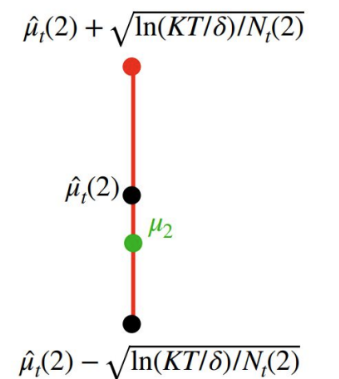
\includegraphics[width =10cm]{Exploration - Regret and Multi-Armed bandits/large_confidence_bound.png}
    \item A small confidence interval indicates that the algorithm has a high degree of confidence in the estimated mean reward for that arm. This happens when an arm has been pulled many times, so the estimate for its reward, $\hat{\mu}_t(i)$, is likely close to the true reward $\mu_t(i)$. As the arm is pulled more frequently, $N_t(i)$ increases and shrinks the interval. If an arm has a small confidence interval, the exploration bonus for that arm is small, meaning the algorithm will exploit this arm more often, choosing it over arms with less accurate estimates. In this case, we prioritize exploitation because we have enough data about this arm to trust its empirical mean. The algorithm assumes that further exploration won’t add much new information. 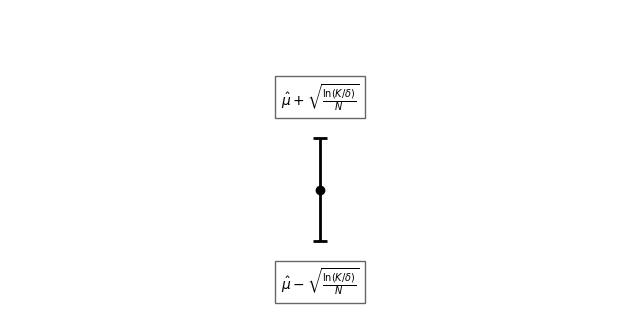
\includegraphics[width =10cm]{Exploration - Regret and Multi-Armed bandits/small_confidence_bound.png}
\end{itemize}


\subsubsection{UCB regret}

Before building the complete regret for the UCB algorithm, we analyze the regret at time $t$. The regret at time $t$ measures the instantaneous regret incurred by selecting the arm $I_t$ at time $t$. It is the difference between the reward of the best possible arm $I^*$ (with the highest true mean reward $\mu^*$) and the reward of the chosen arm $\mu_{I_t}$:

$$
    R(t) = \mu^* - \mu_{I_t}
$$

Using the properties of the UCB algorithm, we can bound this regret by the uncertainty in the empirical mean estimate:

$$
    R(t) \leq \hat{\mu}_t(I_t) + \sqrt{\frac{\ln\left(\frac{KT}{\delta}\right)}{N_t(I_t)}} - \mu_{I_t} \leq 2 \sqrt{\frac{\ln\left(\frac{KT}{\delta}\right)}{N_t(I_t)}}
$$

The total regret over $T$ time steps is the sum of the instantaneous regret over all time steps $t$:

$$
    R(T) = \sum_{t=0}^{T-1} (\mu^* - \mu_{I_t})
$$

By applying the previously found bound for each time step, we get:

$$
    R(T) \leq \sum_{t=0}^{T-1} 2 \sqrt{\frac{\ln\left(\frac{KT}{\delta}\right)}{N_t(I_t)}}
$$

Since the logarithmic term is constant throughout the summation, we can factor it out:

$$
    R(T) \leq 2 \sqrt{\ln\left(\frac{KT}{\delta}\right)} \sum_{t=0}^{T-1} \frac{1}{\sqrt{N_t(I_t)}}
$$

Because we have $K$ different arms, we can group the summation by arm:

$$
    \sum_{t=0}^{T-1} \frac{1}{\sqrt{N_t(I_t)}} = \sum_{i=1}^{K} \sum_{t=0}^{T-1} 1[I_t = i] \frac{1}{\sqrt{N_t(i)}}
$$

Where the indicator function $1[I_t = i]$ is 1 when the $i$-th arm is chosen at time $t$. This clusters the times the $i$-th arm is pulled together. The inner summation can be rewritten as:

$$
    \sum_{i=1}^{K} \sum_{t=1}^{n_T(i)} \frac{1}{\sqrt{t}}
$$

This summation can be bounded by:

$$
    \sum_{i=1}^{K} \sum_{t=1}^{n_T(i)} \frac{1}{\sqrt{t}} \leq \sum_{i=1}^{K} 2 \sqrt{n_T(i)}
$$

We can now perform some mathematical tricks to bound the final regret:

$$
    K \frac{1}{K} \sum_{i=1}^{K} \sqrt{n_T(i)} \leq K \sqrt{\frac{1}{K} \sum_{i=1}^{K} n_T(i)} = K \sqrt{\frac{T}{K}} = \sqrt{KT}
$$

Thus, the total regret for the UCB algorithm is bounded by:

$$
    R(T) \leq 2 \sqrt{\ln\left(\frac{KT}{\delta}\right)} \cdot \sqrt{KT}
$$

This shows that the regret grows sublinearly with the number of trials $T$, meaning that the algorithm performs well over time.